\startAnhang

\listofanhang
\clearpage

\lstset{language=TeX, % hervorzuhebende Keywords definieren
  morekeywords={anhang, anhangteil}
}

\anhang{Docker-Compose Datei}\label{anhang:dockercompose}
\lstinputlisting{includes/compose.yml}

\anhang{Zusätzliche Diagramm-Analysen mit Apache Superset}\label{anhang:zusaetlichediagramme}
\anhangteil{Gehaltsverteilung nach Erfahrungslevel}\label{anhang:1}
\begin{figure}[H]
  \centering
  \captionsetup{list=no} % This line prevents the figure from appearing in the list of tables
  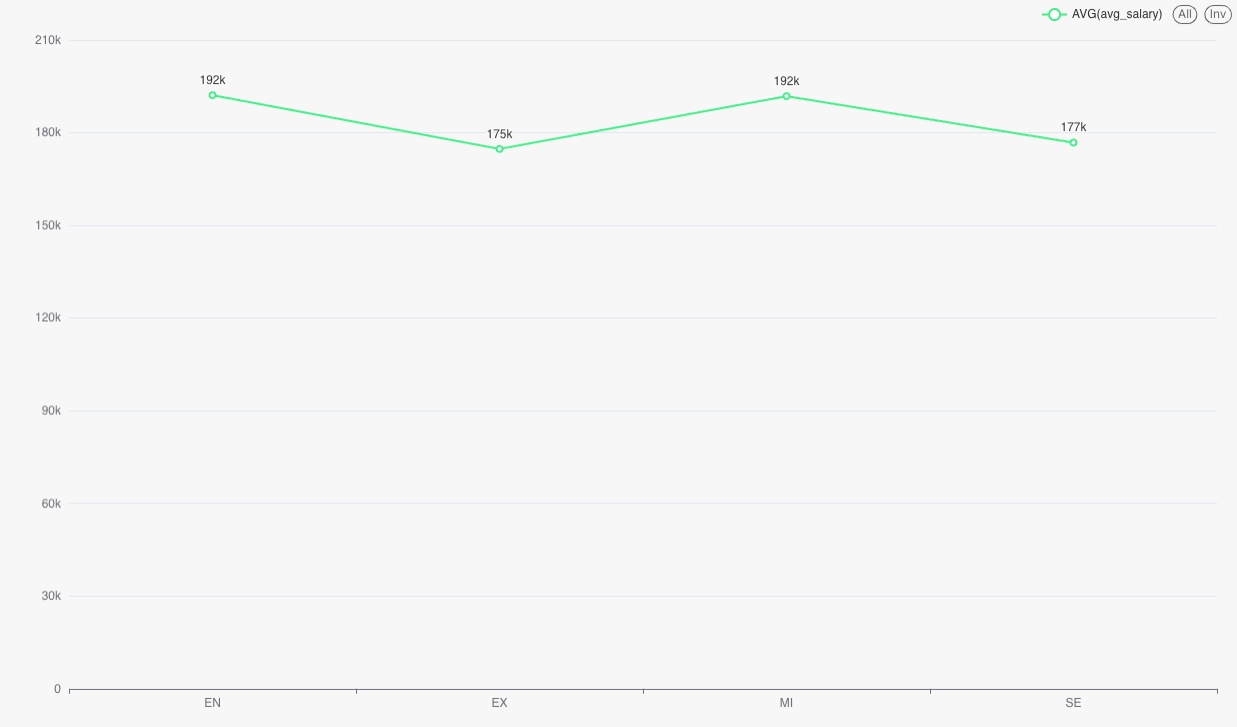
\includegraphics[width=1\linewidth]{graphics/salary-distribution-by-experience-level-2025-01-19T14-55-24.076Z.jpg}
  \caption[Gehaltsverteilung nach Erfahrungslevel]{Gehaltsverteilung nach Erfahrungslevel.}
  \label{fig:chart3}
\end{figure}

\anhangteil{Gehalt im Verhältnis zur prozentualen Remote-Arbeit}\label{anhang:2}
\begin{figure}[H]
  \centering
  \captionsetup{list=no} % This line prevents the figure from appearing in the list of tables
  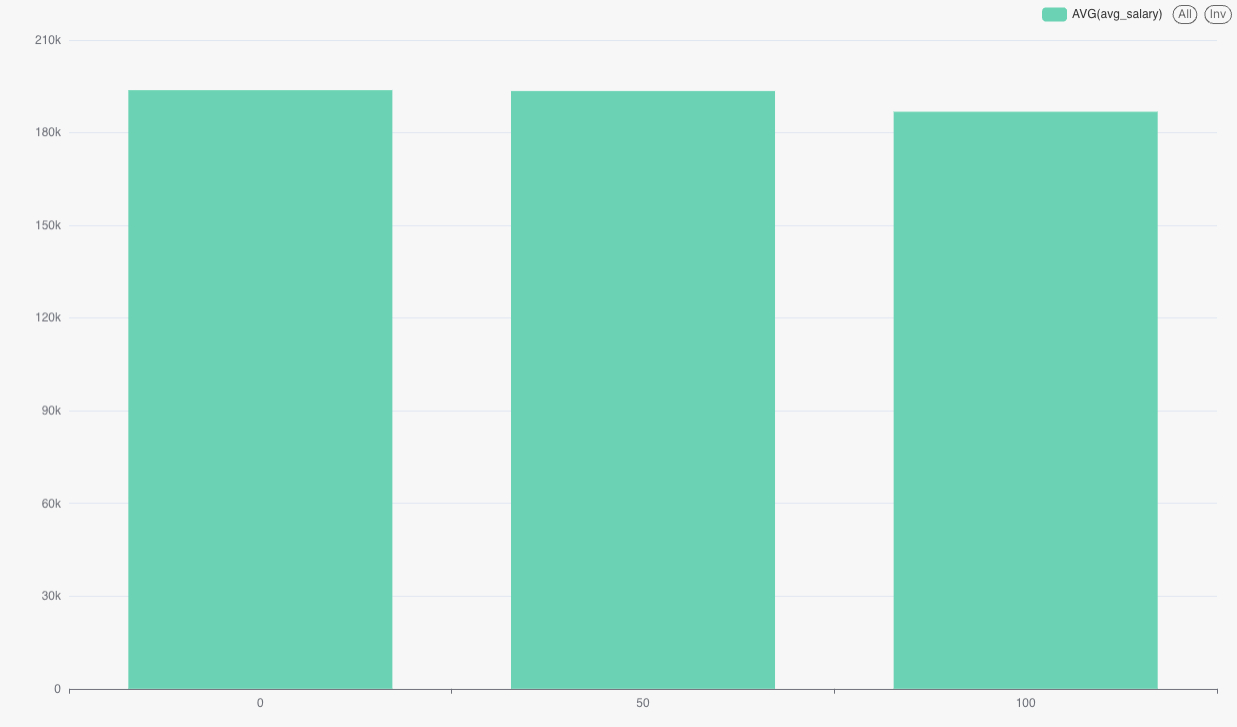
\includegraphics[width=0.8\linewidth]{graphics/salary-remote-ratio.jpg}
  \caption[Gehalt im Verhältnis zur prozentualen Remote-Arbeit]{Gehalt im Verhältnis zur prozentualen Remote-Arbeit.}
  \label{fig:Salary-Remote-Ratio}
\end{figure}

\anhangteil{Representation der Arbeitnehmer nach Unternehmensgröße}\label{anhang:3}
\begin{figure}[H]
  \centering
  \captionsetup{list=no} % This line prevents the figure from appearing in the list of tables
  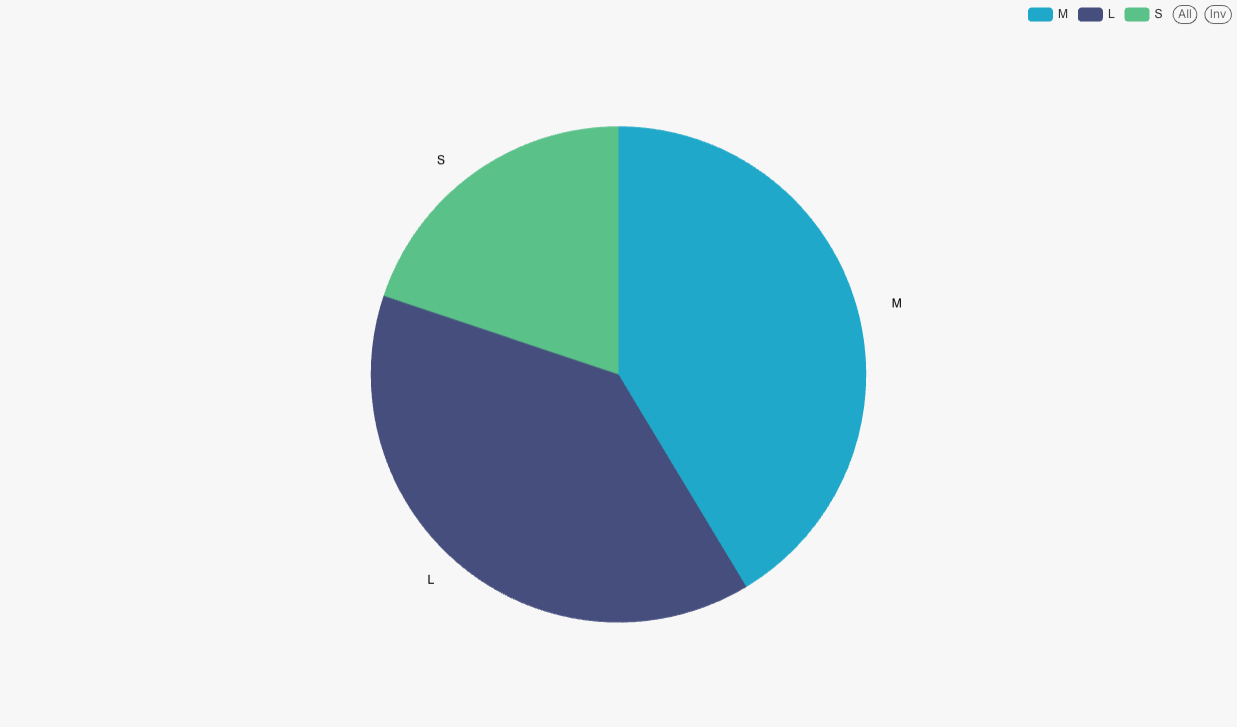
\includegraphics[width=1\linewidth]{graphics/employee-per-company.jpg}
  \caption[Representation der Arbeitnehmer nach Unternehmensgröße aus dem Datensatz]{Representation der Arbeitnehmer nach Unternehmensgröße aus dem Datensatz.}
  \label{fig:chart2}
\end{figure}

\anhang{Core Dump beim erstellen von einem Dashboard in Apache Superset}\label{anhang:apachesuperset}
\begin{figure}[htb]
  \centering
  \captionsetup{list=no} % This line prevents the figure from appearing in the list of tables
  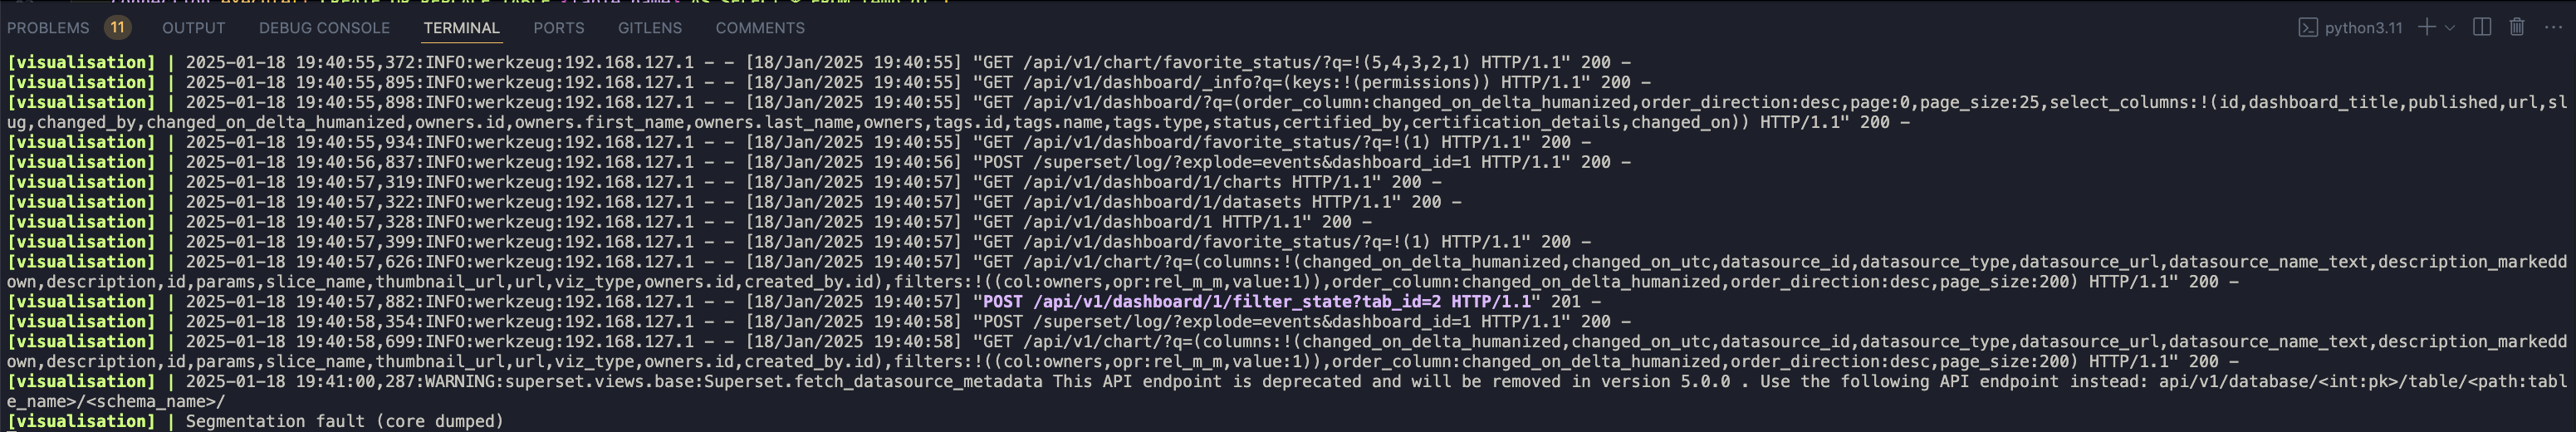
\includegraphics[width=1\linewidth]{graphics/core dump.png}
  \caption[Core Dump beim erstellen von Dashboard in Apache Superset]{Core Dump beim erstellen von Dashboard in Apache Superset. Als Fehlermeldung wird Segmentation fault (core dumped) angezeigt.}
  \label{fig:chart3}
\end{figure}